\chapter{Commandes}

La page est composée d'un bouton pour accéder à la composition d'une nouvelle
commande et de deux tableaux, pour les commandes en cours et les commandes
finalisées.

\paragraph{}

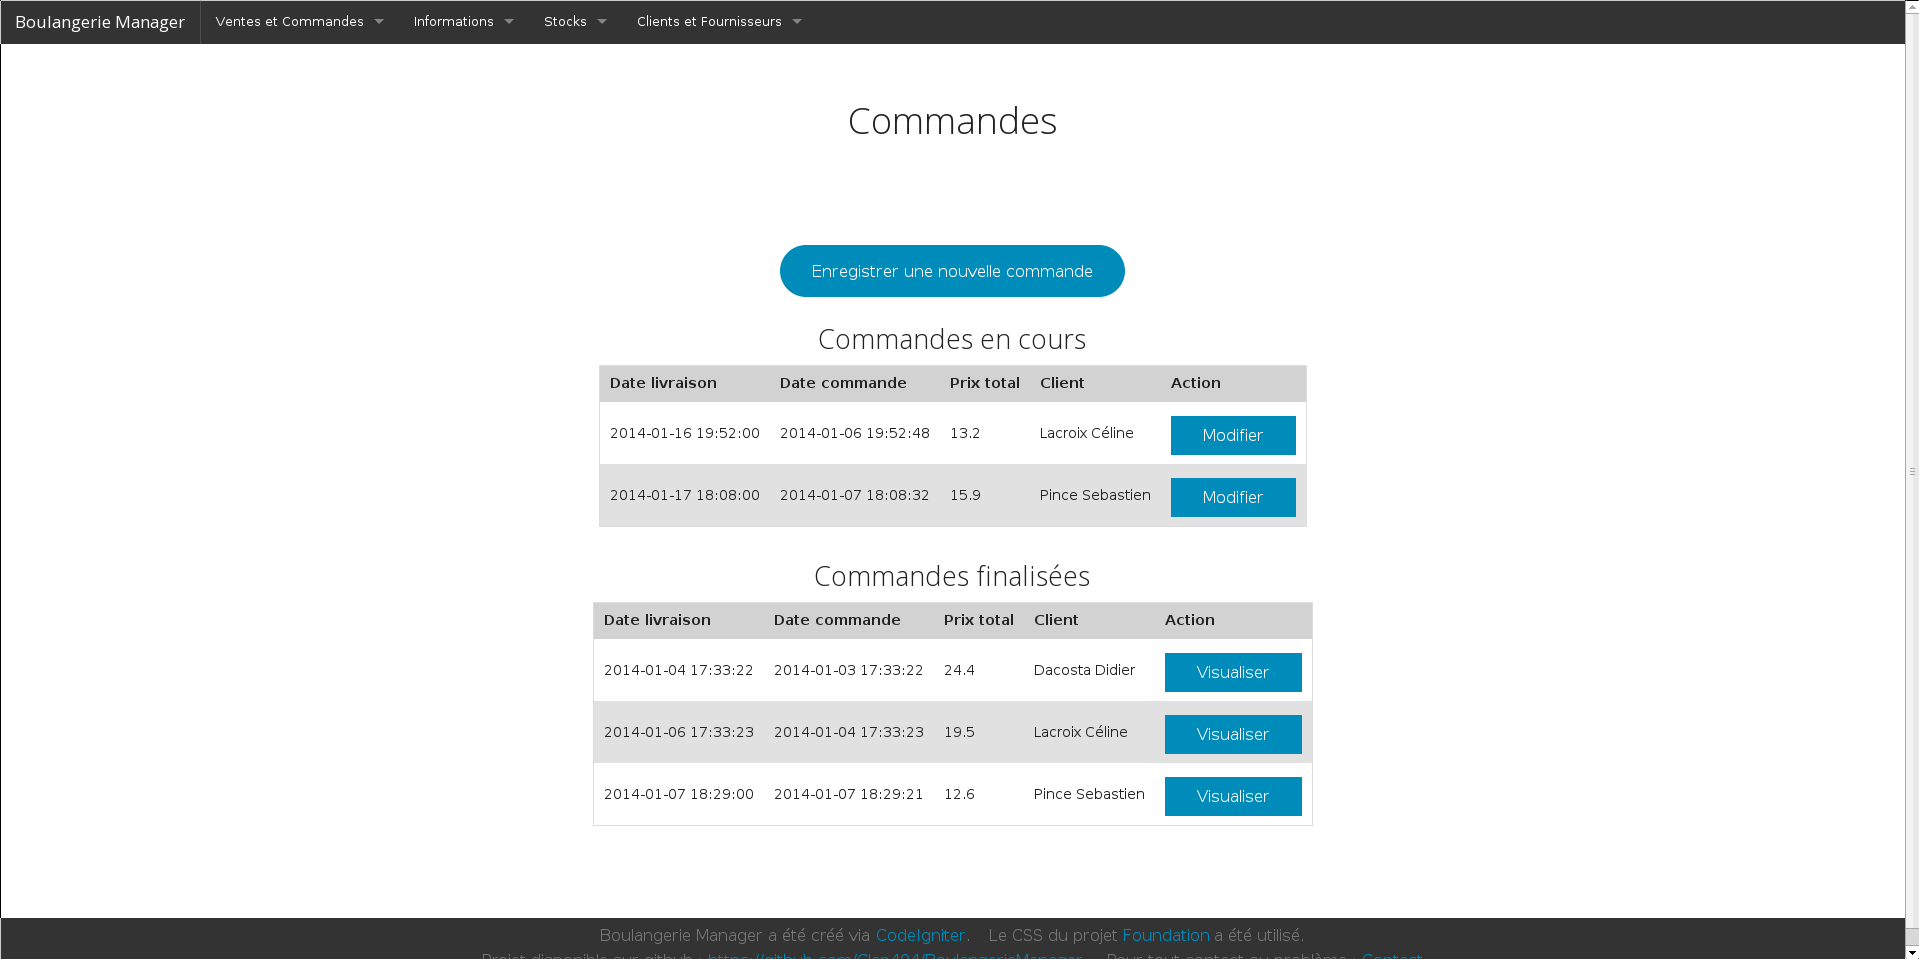
\includegraphics[scale=0.30]{commande1.png}\\

Les commandes sont situées dans "Commandes en cours" ou "Commandes finalisées"
suivant leur date de livraison. Les commandes en cours peuvent encore être
modifiées tandis que les commandes considérées comme finalisées peuvent
seulement être consultées.

\section{Enregistrer une nouvelle commande}

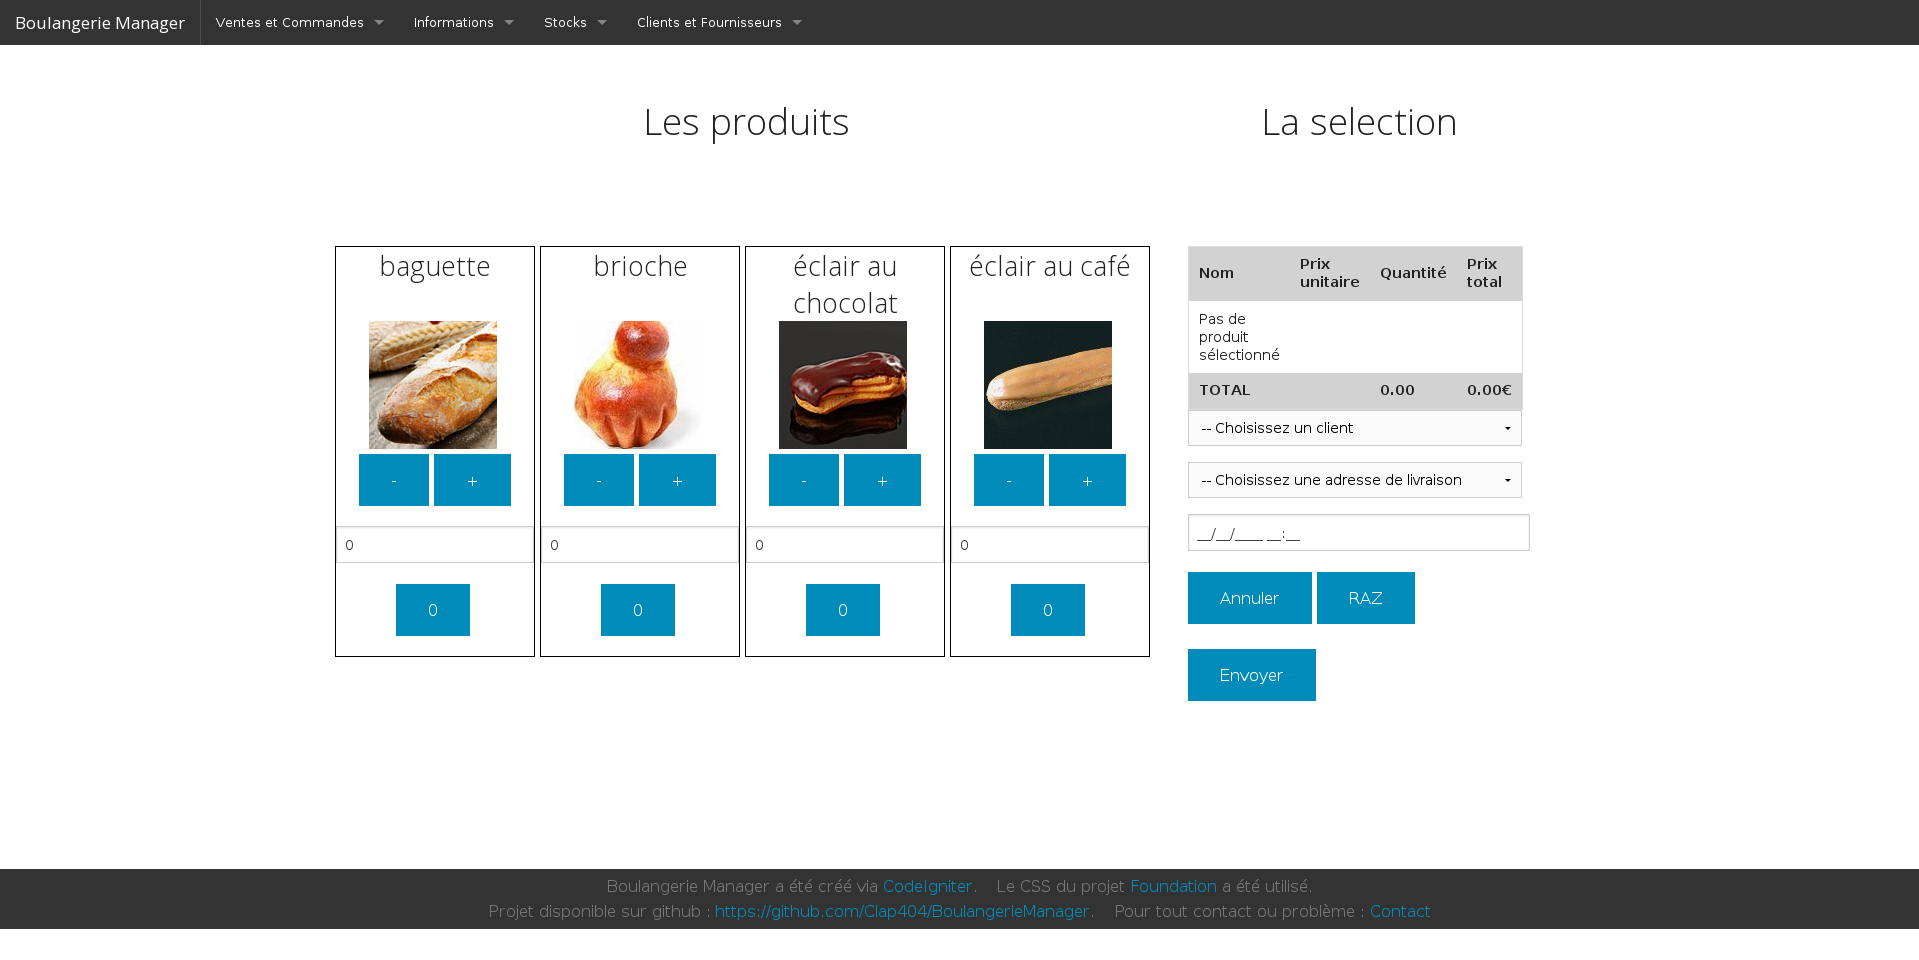
\includegraphics[scale=0.30]{commande2.png}\\

Un clic sur le bouton "Enregistrer une nouvelle commande" ouvre la page de
composition d'une nouvelle commande. Cette page est identique à la page de
composition d'une nouvelle vente, à l'exception de la liste de sélection
d'une adresse de livraison et du sélecteur de la date de livraison.

\paragraph{}
Pour enregistrer une nouvelle commande, commencez par sélectionner un client
dans la liste puis choisissez une adresse de livraison parmi les adresses du
client. Si aucun client n'est sélectionné, aucune adresse ne sera
proposée pour la livraison.

\paragraph{}
Sélectionnez ensuite la date convenue pour la livraison de la commande.
La commande apparaîtra sur la page "Commandes" dans la liste des commandes en
cours jusqu'à la date de livraison où elle passera dans la liste des commandes
finalisées.

\paragraph{}
Dans le cas où vous passez une commande pour un nouveau client ou pour un client
existant à une nouvelle adresse, vous devez d'abord ajouter un client ou ajouter
une adresse comme décrit dans le chapitre "Clients".

\section{Modifier une commande}

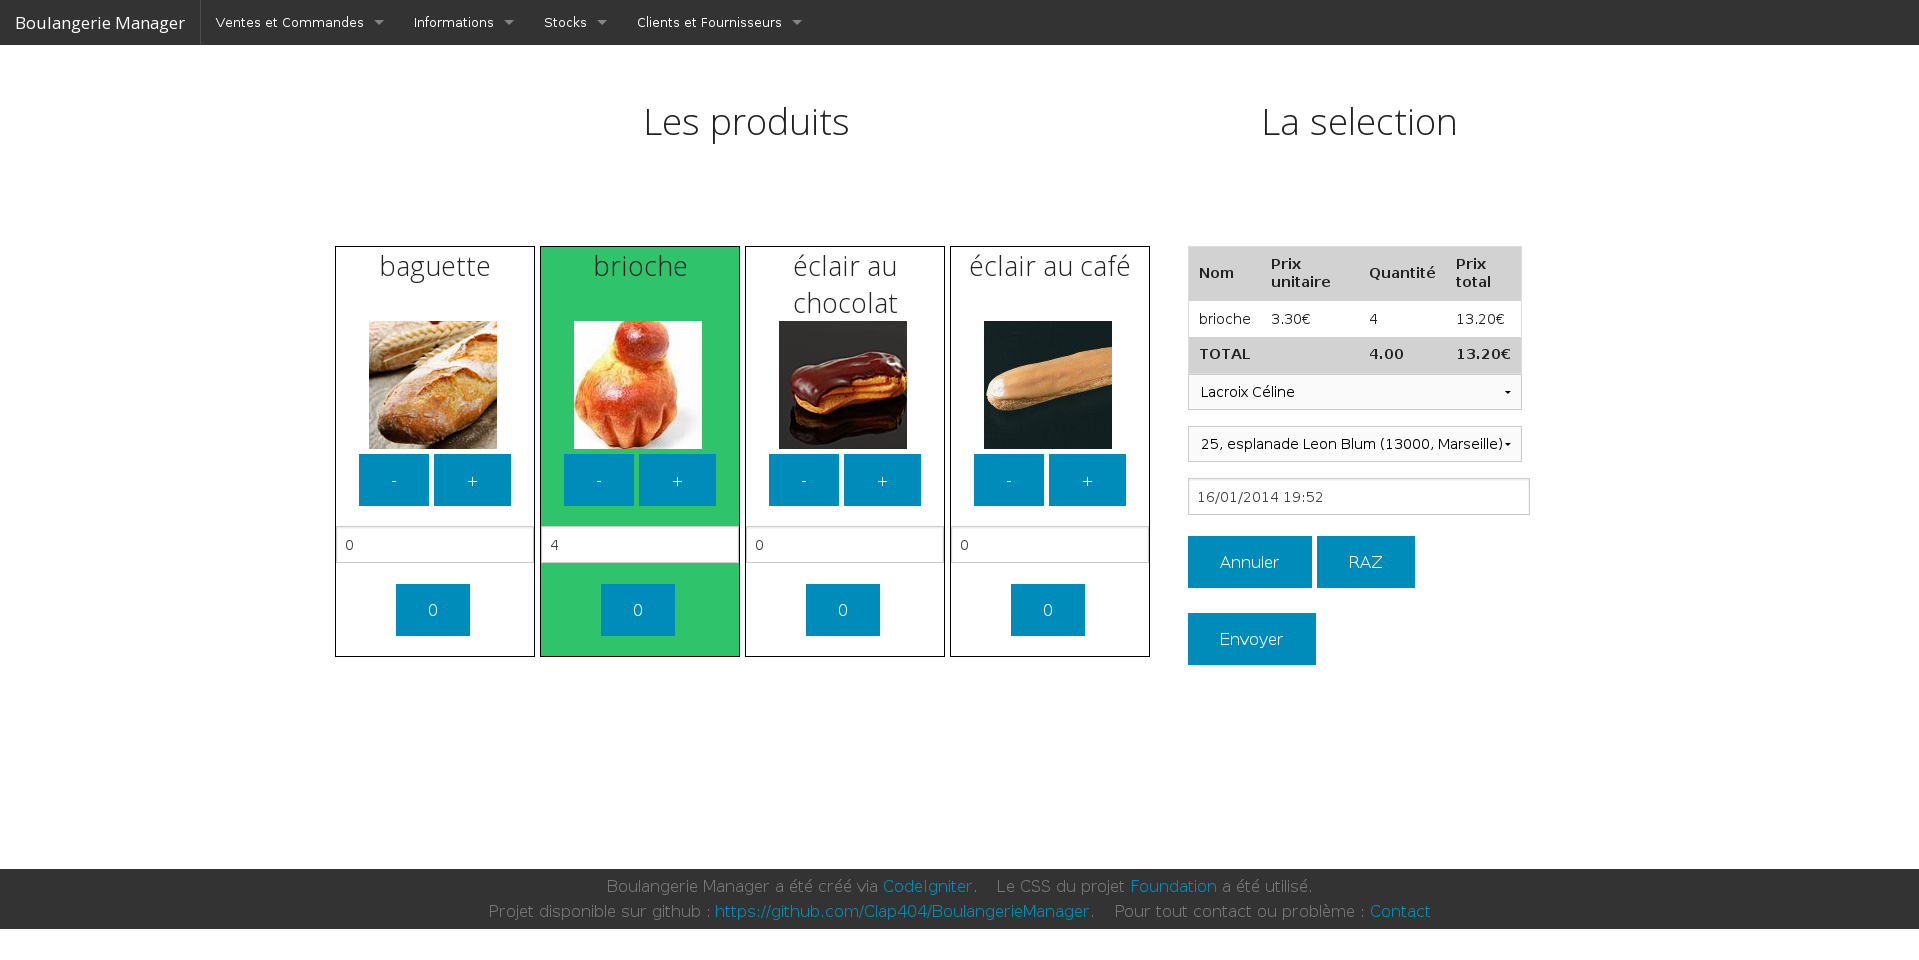
\includegraphics[scale=0.30]{commande3.png}\\

Si vous souhaitez modifier une commande qui n'est pas encore finalisée, il
vous suffit de cliquer sur le bouton "Modifier" placé sur la ligne de la
commande à modifier. Ce bouton rouvre la page de composition d'une commande dans
l'état où vous l'avez enregistrée. Il vous suffit de faire les rectifications
souhaitées avant d'appuyer sur "Envoyer" comme lors de la création d'une
nouvelle commande.

\section{Annuler une commande en cours}
Si vous souhaitez annuler une commande en cours, cliquez sur le bouton
"Modifier" et, une fois sur l'écran de composition de commande, videz simplement
la commande grâce au bouton "RAZ" ("Remise À Zéro") avant de valider.
